\documentclass[11pt]{article}
\usepackage[margin=1in]{geometry}
\usepackage{amsmath,amssymb}
\usepackage{listings}
\usepackage{xcolor}
\usepackage{graphicx}
\usepackage{hyperref}

\lstset{
  basicstyle=\ttfamily\footnotesize,
  breaklines=true,
  frame=single,
  language=C++
}

\begin{document}

\noindent\textbf{ECE 759 --- Assignment 3} \hfill Pranav Mehrotra \\

\vspace{1.5em}

\noindent\textbf{GitHub Link:} \url{https://github.com/pmehrotra3/repo759/tree/main/HW03}

\vspace{1.5em}

\noindent\textbf{Task 1.}\\

\begin{enumerate}
  \item[a)] \texttt{matmul.cpp} (containing \texttt{mmul}, the OpenMP parallel version of \texttt{mmul2} from HW02) present in \texttt{HW03} folder.
  \item[b)] \texttt{task1.cpp} present in \texttt{HW03} folder.
  \item[c)] The plot of the time taken by \texttt{mmul} versus $t$ for $n = 1024$ is shown below.
  \begin{center}
    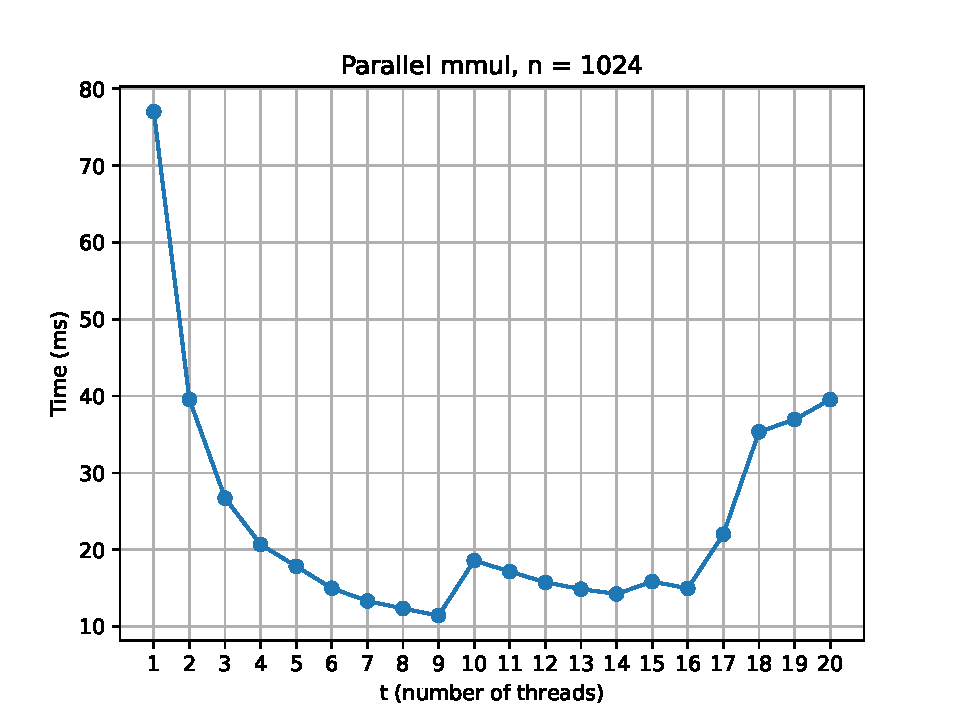
\includegraphics[width=0.7\textwidth]{task1.pdf}
  \end{center}
\end{enumerate}

\newpage
\noindent\textbf{Task 2.}\\

\begin{enumerate}
  \item[a)] \texttt{convolution.cpp} present in \texttt{HW03} folder.
  \item[b)] \texttt{task2.cpp} present in \texttt{HW03} folder.
  \item[c)] The plot of the time taken by \texttt{convolve} versus $t$ for $n = 1024$ is shown below.
  \begin{center}
    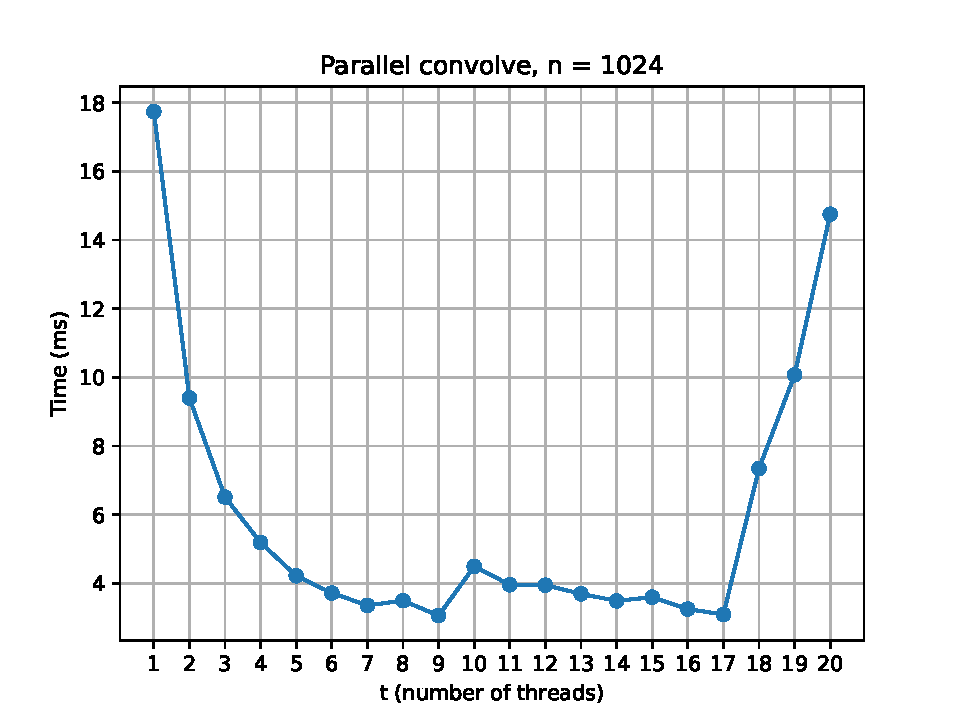
\includegraphics[width=0.7\textwidth]{task2.pdf}
  \end{center}
  Adding threads improves performance only up to a point: the time drops from 17.7 ms with 1 thread to about 3.1 ms with 9 threads as the workload is divided among them. Beyond that point, performance stops improving because the overhead of creating, managing, and synchronizing the extra threads cancels out the benefit of parallelism.
\end{enumerate}

\newpage
\noindent\textbf{Task 3.}\\

\begin{enumerate}
  \item[a)] \texttt{msort.cpp} (parallel merge sort using OpenMP tasks, with insertion sort below the threshold) present in \texttt{HW03} folder.
  \item[b)] \texttt{task3.cpp} present in \texttt{HW03} folder.
  \item[c)] The plot of the time taken by \texttt{msort} versus \texttt{ts} for $n = 10^6$ and $t = 8$ is shown below. The best threshold was $\texttt{ts} = 128$.
  \begin{center}
    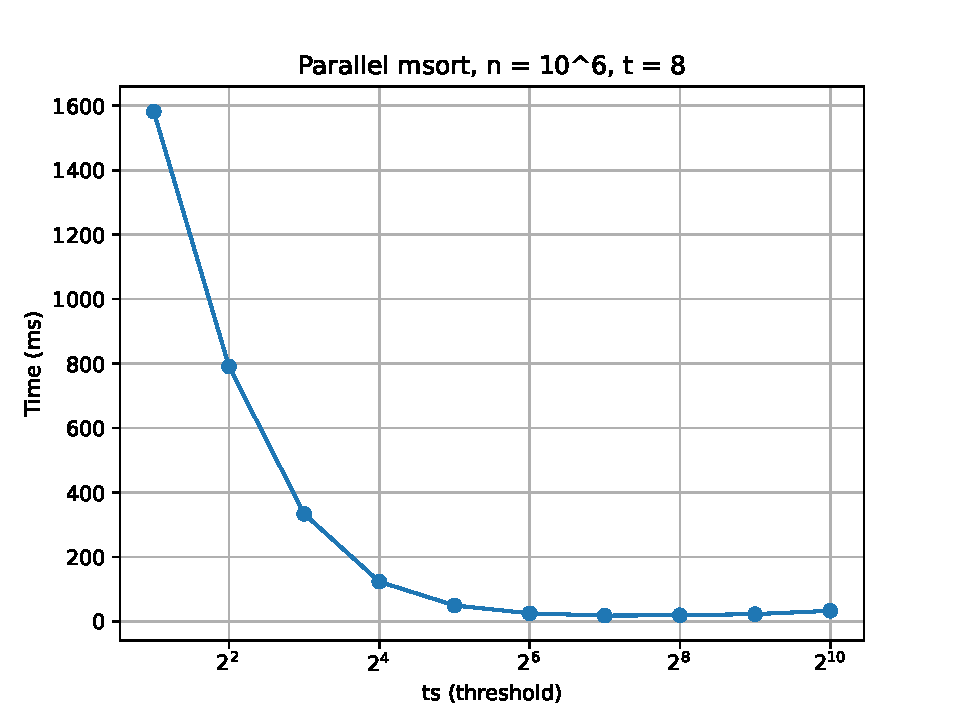
\includegraphics[width=0.55\textwidth]{task3_ts.pdf}
  \end{center}
  The plot of the time taken by \texttt{msort} versus $t$ for $n = 10^6$ and $\texttt{ts} = 128$ is shown below.
  \begin{center}
    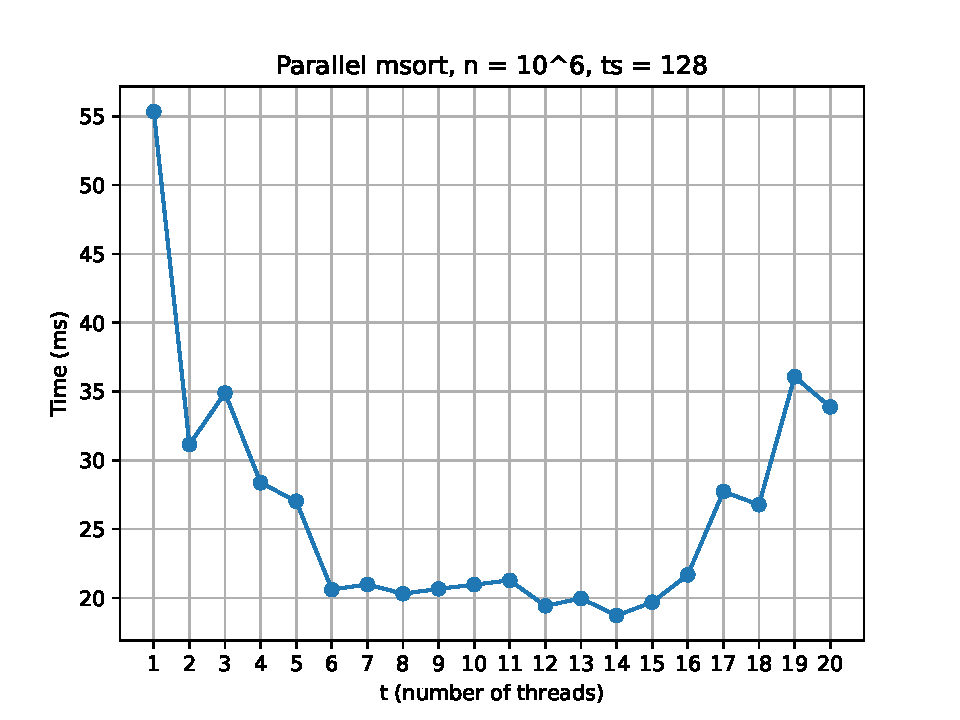
\includegraphics[width=0.55\textwidth]{task3_t.pdf}
  \end{center}
\end{enumerate}

\end{document}
